\colorlet{circle edge}{black!50}
\colorlet{circle area}{gray!20}

\tikzset{
  filled/.style={fill=circle area, draw=circle edge, thick},
  outline/.style={draw=circle edge, thick}
  }

\setlength{\parskip}{5mm}

\tikzstyle{edge} = [draw, thick, -]
\tikzstyle{vertex}=[circle,fill=black!50,minimum size=10pt,inner sep=0pt]
\tikzstyle{selected edge} = [draw, line width=2cm,-,gray!20] 
\tikzstyle{real edge} = [draw, line width=8pt,-, gray!70]

\subfloat[Graph with transmission radius]{\label{fig:trans}
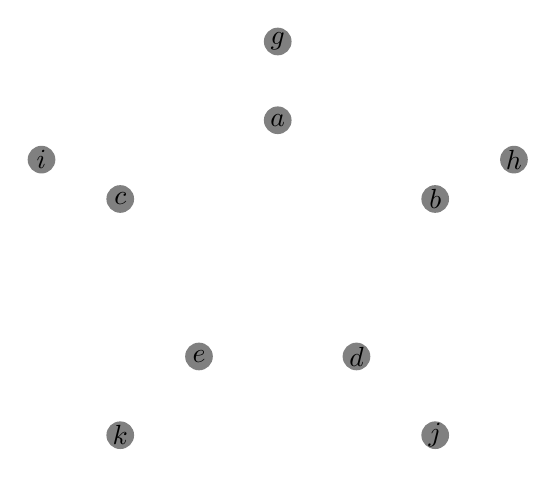
\begin{tikzpicture}  
    
       \foreach \pos/\name in {{(0,2)/a}, {(2,1)/b}, {(-2,1)/c}, {(1,-1)/d}, {(-1,-1)/e}, {(0,3)/g}, {(3,1.5)/h}, {(-3, 1.5)/i}, {(2,-2)/j}, {(-2,-2)/k}} {
           \node[vertex] (\name) at \pos {$\name$};
       }

\end{tikzpicture}}
\subfloat[Connection graph]{\label{fig:connec}
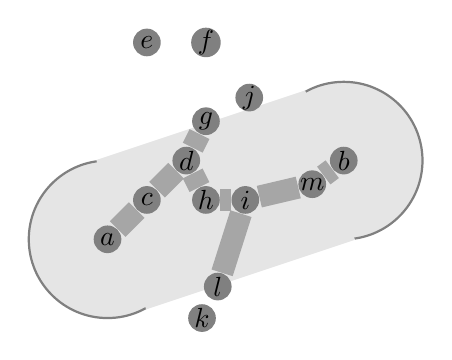
\begin{tikzpicture}  
    % Definition of the radii
    \def\firstradius{(0,0) circle (1cm)};
    \def\secondradius{(3, 1) circle (1cm)};

    \fill[filled] \firstradius;
    \fill[filled] \secondradius;
    
     % The real source and sink
    \foreach \pos/\name in {{(0,0)/a}, {(3, 1)/b}} {   
      \node[vertex] (\name) at \pos {$\name$};
    }
   
    \path[selected edge] (a) -- (b);

    % the extra nodes
    \foreach \pos/\name in {{(0.5,0.5)/c}, {(1,1)/d}, {(0.5, 2.5)/e}, {(1.25, 2.5)/f}, {(1.25, 1.5)/g}, {(1.25, 0.5 )/h}, {(1.75, 0.5)/i}, {(1.80, 1.8)/j}, {(1.20, -1)/k}, {(1.40, -0.6)/l}, {(2.6, 0.7)/m}} {   
      \node[vertex] (\name) at \pos {$\name$};
    }

    % The connections between them
    \foreach \source/\sink in {a/c, c/d, d/h, h/i, i/m, m/b, i/l, d/g} {
      \path[real edge] (\source) -- (\sink);
    }


\end{tikzpicture}}
% Remove empty line
\subfloat[Routing graph]{\label{fig:routing}
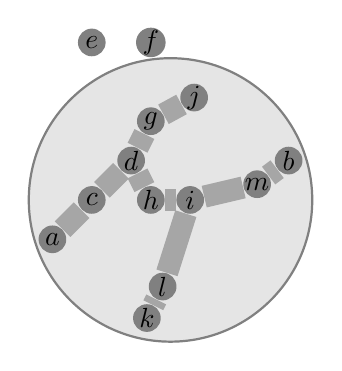
\begin{tikzpicture}  

    % Definition of the radii
    \def\radius{(1.5,0.5) circle (1.8)};
    \fill[filled] \radius;

     % The real source and sink
    \foreach \pos/\name in {{(0,0)/a}, {(3, 1)/b}} {   
      \node[vertex] (\name) at \pos {$\name$};
    }
   
    % the extra nodes
    \foreach \pos/\name in {{(0.5,0.5)/c}, {(1,1)/d}, {(0.5, 2.5)/e}, {(1.25, 2.5)/f}, {(1.25, 1.5)/g}, {(1.25, 0.5 )/h}, {(1.75, 0.5)/i}, {(1.80, 1.8)/j}, {(1.20, -1)/k}, {(1.40, -0.6)/l}, {(2.6, 0.7)/m}} {   
      \node[vertex] (\name) at \pos {$\name$};
    }

    % The connections between them
   \foreach \source/\sink in {a/c, c/d, d/h, h/i, i/m, m/b, i/l, d/g, g/j, l/k} {
      \path[real edge] (\source) -- (\sink);
    } 
\end{tikzpicture}}
